\chapter{Linking modern coexistence theory and contemporary niche theory}
%\chaptermark{Niche and coexistence theory}
%\renewcommand{\sectionmark}[1]{}
\fancyhead[LE, RO]{\thepage}
\fancyhead[RE]{CHAPTER 2}
\fancyhead[LO]{NICHE AND COEXISTENCE THEORY}
\fancyfoot{}
\renewcommand{\headrulewidth}{0pt}
\setlength{\parindent}{1cm}


\begin{comment}
\documentclass[hidelinks,12pt]{article}
\usepackage{graphicx,bm, booktabs,lineno,array}
\usepackage[fleqn]{amsmath}
\setlength{\mathindent}{0pt}
\usepackage[compress,comma]{natbib}
\usepackage[a4paper]{geometry}
\usepackage[parfill]{parskip}
\usepackage[usenames,dvipsnames]{color}
\usepackage[font=large,labelfont=bf,margin=1cm, labelsep = none]{caption} % caption formatting
\usepackage{setspace}
\usepackage{gensymb}
\usepackage{color} 
\usepackage{sidecap}
\usepackage{etoolbox}
\newbool{MyRefNumbers}
\usepackage{authblk}
\usepackage{hyperref}
\usepackage[color=cyan]{todonotes}
\pdfminorversion=3
\doublespacing

\newcommand{\plus}{\raisebox{.4\height}{\scalebox{.6}{+}}}
\newcommand{\minus}{\raisebox{.4\height}{\scalebox{.8}{-}}}
\newcommand*\samethanks[1][\value{footnote}]{\footnotemark[#1]}
\newcommand\blfootnote[1]{%
  \begingroup
  \renewcommand\thefootnote{}\footnote{#1}%
  \addtocounter{footnote}{-1}%
  \endgroup
}
\end{comment}



\begin{comment}
\title{Linking modern coexistence theory and contemporary niche theory}
\author[1]{Andrew D. Letten \thanks{These authors contributed equally.}}
\author[1]{Po-Ju Ke \samethanks}
\author[1]{Tadashi Fukami}
\affil[1]{Department of Biology, Stanford University, Stanford, California, 94305-5020, USA}

\begin{document}

\date{}
\maketitle
\singlespacing
\blfootnote{Correspondence email: aletten@stanford.edu, pojuke@stanford.edu, fukamit@stanford.edu}
\textbf{Type of article:} Concepts and Synthesis
\textbf{Running title:} Niche and coexistence theory 
\textbf{Figures:} 6\\
\textbf{Boxes:} 2\\
\newpage
\doublespacing
\linenumbers
\end{comment}



\section{Abstract}
Modern coexistence theory and contemporary niche theory represent parallel frameworks for understanding the niche's role in species coexistence. Despite increasing prominence and shared goals, their compatibility and complementarity have received little attention. This paucity of overlap not only presents an obstacle to newcomers to the field, but it also precludes further conceptual advances at their interface. Here, we present a synthetic treatment of the two frameworks. We review their main concepts and explore their theoretical and empirical relationship, focusing on how the resource supply ratio, impact niche, and requirement niche of contemporary niche theory translate into the stabilizing and equalizing processes of modern coexistence theory. We show for a general consumer-resource model that varying resource supply ratios reflects an equalizing process; varying impact niche overlap reflects a stabilizing process; and varying requirement niche overlap may be both stabilizing and equalizing, but has no qualitative effect on coexistence. These generalizations provide mechanistic insight into modern coexistence theory, while also clarifying the role of contemporary niche theory's impacts and requirements in mediating coexistence. From an empirical perspective, we recommend a hierarchical approach, in which quantification of the strength of stabilizing mechanisms is used to guide more focused investigation into the underlying niche factors determining species coexistence. Future research that considers alternative assumptions, including different forms of species interaction, spatio-temporal heterogeneity, and priority effects, would facilitate a more complete synthesis of the two frameworks.
\medskip


\textbf{Keywords:} mechanistic models, coexistence, competition, consumer-resource, fitness differences, niche overlap, impact niche, requirement niche, Lotka--Volterra



\section{Introduction}
The niche concept has an unstable history in community ecology. As recently as the turn of this century, Hubbell's unified neutral theory \citep{Hubbell2001} came close to rendering the concept and its overburdened assortment of models, mechanisms, and processes largely obsolete. Yet over the past 10-15 years the niche has enjoyed a return to vogue. This is thanks in no small part to the independent development of two distinct frameworks for identifying the niche's role in species coexistence. The first of these, referred to here and elsewhere as ``contemporary niche theory", has its origins in the mechanistic consumer-resource models pioneered by \citet{MacArthur1970}, popularised by \citet{tilman1982}, and extended by \citet{Chase2003}, among others. Following a similar nomenclature, the second,  ``modern coexistence theory" \citep{Chesson2000, Adler2007, Hillerislambers2012}, is more closely allied to the phenomenological Lotka--Volterra models familiar to all students of ecology. The emergence of these two frameworks has revitalized the field, and yet despite shared goals, their compatibility and complementarity has received little attention. Of the 2300+ citations (since 2003) of Chesson's \citeyear{Chesson2000} paper formalizing modern coexistence theory, only $\sim$180 also cite contemporary niche theory's primary text \citep{Chase2003}, while of the 1250+ citing the latter only $\sim$200 also cite the former. The paucity of overlap not only presents an obstacle to newcomers to the field seeking an entry point to the study of species coexistence, but it also precludes further conceptual advances taking advantage of the strengths of each. Here we offer a synthesis of contemporary niche theory and modern coexistence theory that strives to do both.
\par


MacArthur's first forays into mechanistic models of competition were motivated by a desire to make the ecological processes behind Lotka--Volterra competition dynamics more transparent \citep{MacArthur1964, MacArthur1970, macarthur1972}. The cost of translating Lotka--Volterra competition coefficients into consumer-resource dynamics was the need to make a series of assumptions about the processes and factors involved \citep{Chesson1990}. This trade-off between mechanistic precision (e.g., which resources are regulating coexistence?) and phenomenological accuracy (e.g., can they coexist?) has been inherited by the two frameworks discussed here. Inference using contemporary niche theory is limited by the investigators' knowledge of the natural history of system. On the other hand, the mathematically abstracted emergent properties of modern coexistence theory can all but obscure the underlying ecology. As yet, modern coexistence theory lacks an intuitive conceptual framework for translating the traits and life-history of interacting species into the niche overlap and fitness difference terms (see below) used to quantify coexistence. The few empirical studies to tackle this problem have largely documented weak or complex relationships between interacting species' niche and fitness differences and their evolutionary relatedness or functional similarity \citep{Narwani2013, Godoy2014, Kraft2015, Germain2016}.
\par


A complementary pathway to the demystification of modern coexistence theory is to explore its relationship with the mechanistic framework of contemporary niche theory, which can provide a more explicit connection between species traits and the outcomes of competitive interactions. In an early paper foreshadowing the development of modern coexistence theory, \citet{Chesson1990} showed how his niche overlap and fitness difference terms could be quantified directly from the parameters of MacArthur's consumer-resource model. More recently, \citet{Kleinhesselink2015} have shown how Chesson's niche overlap could be derived from Tilman's (\citeyear{tilman1982}) consumer resource model. Nevertheless, to our knowledge, there has been no previous work explicitly examining how the criteria for coexistence under contemporary niche theory translate into both the niche overlap and fitness difference terms of modern coexistence theory.
\par


A synthetic treatment of the two frameworks necessarily begins with an introduction to their fundamentals. In the interest of space, we have kept this section concise, and refer readers to several earlier articles and books for a more nuanced unpacking of their respective origins and development (e.g., contemporary niche theory: \citealp{tilman1982, Grover1997, Chase2003}; modern coexistence theory: \citealp{Chesson2000, Adler2007, Hillerislambers2012, Chesson2013ecosys}). This section is followed by an analytical exploration of the relationship between the two frameworks, complemented by analyses using empirical data from the literature. In the penultimate section, we discuss the relative merits of each framework in an empirical context. Finally, we conclude by highlighting some future directions and opportunities. 
\par



\section{Modern coexistence theory and the niche}
Under modern coexistence theory, two different classes of mechanisms mediate coexistence: equalizing mechanisms that reduce the average fitness difference between species; and stabilizing mechanisms that reduce niche overlap. Although equalizing and stabilizing mechanisms can theoretically be defined for any underlying model, here we show how they can be understood using a phenomenological Lotka--Volterra model. Under Lotka--Volterra, the complexity of organismal interactions is reduced to summary parameters (competition coefficients) that capture intra- and inter-specific effects on per capita growth rate. When Lotka--Volterra competition is parameterised for two species in terms of absolute competition coefficients (as opposed to carrying capacities and relative competition coefficients), the per capita growth rate of each species can be represented as:

\begin{equation}
\frac{1}{N_{i}}\frac{dN_{i}}{dt} = r_{i}(1 - \alpha_{ii}N_{i} - \alpha_{ij}N_{j}) 
\tag{2.1}\label{eq:2.1}
\end{equation}

\noindent where $r_{i}$ is the maximum per capita growth of species \textit{i}, and $\alpha_{ij}$ represents the impact of species \textit{j} on the per capita growth rate of species \textit{i}. Thus $\alpha_{ii}$ and $\alpha_{ij}$ represent the absolute intra- and inter-specific competition coefficients, respectively. Two species can coexist when $\alpha_{11} > \alpha_{21}$ and $\alpha_{22} > \alpha_{12}$. This pair of inequalities, sometimes referred to as the mutual invasibility criterion, means that for stable coexistence each species must reduce its own growth more than it does that of its competitor. 
\par


Chesson's key insight was that the mutual invasibility criterion can be defined in terms that quantify the degree of niche overlap, $\rho$, between species and their differences in average fitness, $f_{2}/f_{1}$ \citep{Chesson2000}. Specifically, the ratio of inter-specific to intra-specific competition coefficients is equal to the product of a niche overlap term and a fitness ratio term,

\begin{equation}
\frac{\alpha_{12}}{\alpha_{22}} = \frac{f_{2}}{f_{1}} \rho. 
\tag{2.2}\label{eq:2.2}
\end{equation}

\noindent In Chesson's framework, niche overlap, $\rho$, is a measure of the relative strength of intra- to inter-specific density dependence, where differentiation in resource use (or shared predators in the case of apparent competition) leads to low values of $\rho$. When $\rho$ = 0 for a pair of species, they share none of the same resources, or use them completely independently in space and time, and therefore impose no density dependent feedbacks on each other \citep{Chesson2000, Chesson2008}. In contrast, when species' resource use overlaps completely and each resource is of the same relative value to each species, $\rho$ = 1. This definition removes the overall level of adaptedness to the environment from niche comparisons. Instead, this is captured by the fitness ratio, $f_{2}/f_{1}$, which predicts the winner in competition under the hypothetical scenario of complete niche overlap. Note the fitness ratio is also commonly written as $k_{2}/k_{1}$ but we use lower case $f$ to avoid confusion with Lotka--Volterra carrying capacity, $K$.
\par


From the mutual invasibility criterion, we know that the right hand side of the equation above must be less than 1 for species 1 to be able to invade a population of species 2 at equilibrium. This is the same as saying $f_{2}/f_{1} < 1/\rho$. By the same logic, for species 2 to be able to invade a population of species 1, $f_{1}/f_{2} < 1/\rho$. Therefore, satisfaction of the mutual invasibility criterion, i.e., stable coexistence, requires:

\begin{equation}
\rho < \frac{f_{2}}{f_{1}} < \frac{1}{\rho}. 
\tag{2.3}\label{eq:2.3}
\end{equation}

\noindent As $\rho$ goes to 1, the potential for two species to coexist is contingent on increasingly smaller fitness differences between them. Thus we can define an equalizing mechanism as any process that reduces the average fitness difference between species; and a stabilizing mechanism as any process that reduces niche overlap and therefore increases negative frequency dependence (Fig. \ref{fig:conceptfig}a). Stabilizing mechanisms are what cause a species at high density to buffer its own growth more than that of a competitor, while also allowing it to recover from low density due to low inter-specific competition. An example of a stabilizing mechanism would be coexisting plant species acquiring resources from different depths, assuming that the supply of resources is independent \citep{Levine2009}. By contrast, an example of an equalizing mechanism would be a reduction in fitness differences due to an otherwise competitively dominant species experiencing higher density-independent rates of predation or infection by pathogens \citep{Mordecai2011}. Most of the relevant research on the relative strength of stabilizing and equalizing mechanisms has focused on grassland plants as an empirical system \citep[e.g.,][]{Levine2009, Angert2009, Adler2010, Godoy2014, Germain2016}, but work in other systems has also begun to emerge, including arthropods \citep{Siepielski2011}, green algae \citep{Narwani2013} and bacteria \citep{Zhao2015}.
\par
 
 
 
\section{Coexistence and contemporary niche theory}
In their 2003 book, \citet{Chase2003} introduced contemporary niche theory as a synthesis of historically incompatible niche definitions. This they achieved through a conceptual extension of the graphical approach to the analysis of consumer-resource models popularised by \citet{tilman1982}. Unlike phenomenological Lotka--Volterra models, consumer-resource models provide an explicit basis for coexistence. Tilman focused largely on the dynamics of consumer-resource systems, but \cite{Chase2003} showed how the graphical approach could be extended beyond consumer-resource dynamics to incorporate a broad spectrum of biotic and abiotic interactions. Thus, in addition to explaining the coexistence of consumers competing for limiting resources (e.g., algae competing for basic nutrients [Tilman, \citeyear{Tilman1977, tilman1982}] or invertebrates competing for algae [Rothhaupt, \citeyear{Rothhaupt1988}]), contemporary niche theory can be invoked to explain community dynamics arising from a range of alternative niche factors (e.g., the response of marine bacteria to different stressors [Materna \textit{et al.}, \citeyear{Materna2012}], or the sensitivity of plants to the relative abundance of different pollinators, [Pauw \citeyear{Pauw2013}]).  
\par


\citet{Chase2003} redefined the consumption vectors of Tilman as the impact niche,  encompassing not only the impact of consumers on resources, but also their potential impact on other factors such as the density of predators, pathogens or toxic chemicals \citep[see also][]{Grover1997}. The impact niche can then be thought of as representing a species' Eltonian niche \citep{Elton1927}, i.e., the impact a species has on its environment. Similarly, \citet{Chase2003} suggested that the zero net growth isoclines (ZNGIs), which delineate the range of conditions in which a species maintains a positive growth rate, need not be defined only with respect to consumable resources, but could be represented by, for example, the density of predators or the frequency of disturbance. Thus the ZNGIs can be considered akin to the Grinellian or Hutchinsonian view of the niche \citep{10.2307/4072271, hutchinson1957cold}, i.e., the biotic and abiotic requirements of a species, which Chase and Leibold (2003) refer to as the requirement niche, following their earlier work \citep{Leibold1995}.
\par


Under the mechanistic framework of contemporary niche theory, the conditions for local coexistence depend on three criteria (Fig. \ref{fig:conceptfig}b). Notwithstanding the broad scope of the framework, for heuristic purposes, we focus on the simplest and most well studied scenario: two species competing for two limiting resources in a spatially and temporally homogenous environment. First, their ZNGIs must intersect, the ecological implications of which is that each species is a better competitor for a different resource. Second, each species must have a relatively greater impact on the resource it finds most limiting. Third, the supply ratio of the two resources must not disproportionately favour one species over the other. More precisely, the supply ratio must be intermediate to the inverse of the impact vectors (the consumption vectors in a consumer-resource model).
\par


The second of these criteria is perhaps the most familiar in that it is the basis for negative frequency dependent growth and therefore critical to coexistence. However, it is also the most easily misunderstood. A source of confusion is the conventional reference to the `most limiting' resource, which although transparent in the case of essential resources (e.g., the inorganic nutrients obtained separately by plants [N, P, K etc.]), is less clear with respect to substitutable resources (e.g., the more complex food forms consumed by animals). If we define the minimum resource value a species needs to maintain a positive growth rate as its $R^{*}$ \citep[\textit{sensu}][]{tilman1982}, then for essential resources, the most limiting resource is the one for which a species has the higher $R^{*}$. However, if two resources are perfectly substitutable and a consumer can compensate for the complete absence of one resource by the consumption of another, then neither resource is physiologically limiting in the way we think of for plants consuming essential resources. So what is meant by most limiting? As best articulated by \citet{leon1975}, we suggest that an intuitive way to think about this criterion of coexistence is that each competitor must have a greater impact on the resource for which a reduction would have a greater impact on its growth. For substitutable resources it corresponds to the resource for which a species has the \textit{lower} $R^{*}$. Note this runs counter to Fig. 2.8 of \citet[][see also discussion on p. 34]{Chase2003}, but is consistent with \citet{Leibold1998}.    
\par



\section{Disentangling definitions of niche overlap}
Clearly the niche is central to both frameworks, but there are important subtle differences. Under contemporary niche theory, the impact niche and requirement niche can be understood as species-specific properties that are comparable across species. With respect to the impact niche, the cosine of the angle between the two impact vectors in Tilman's consumer-resource models is equivalent to Pianka's (\citeyear{Pianka1973}) measure of niche overlap \citep{Petraitis1989}. With respect to the requirement niche, an explicit measure of niche overlap has yet to be defined, but a heuristic two dimensional definition that we adopt here is the cosine of the angle between the ZNGIs for substitutable resources, and the cosine of the angle between two lines from the origin to the corner of each ZNGI for essential resources.
\par


Under modern coexistence theory, the niche can only be understood in light of species interactions. It cannot be quantified for an individual species in isolation from other species. Instead, the niche is a property of pairwise or one-to-many comparisons between species, and therefore is only defined in terms of niche overlap or niche differences (1 - $\rho$). Further, it is concerned solely with those aspects of species' ecology that generate negative frequency dependence. The exclusion of overall fitness from this niche definition may seem contrary to intuitive species-specific interpretations of the niche (e.g., in species distribution modelling); for instance, two species within a guild that are adapted to high temperature environments will not necessarily exhibit niche overlap in Chesson's framework. Nevertheless, if their fitness equivalence derives from a common adaptation to a limiting resource, they will also exhibit high niche overlap. For example, oligotrophically adapted plants may be expected to exhibit high niche overlap for the very same reason they have high fitness in nutrient poor environments. Chesson's niche overlap is not equivalent to either the impact or requirement niche of contemporary niche theory. However, they are still related, as we now show. 
\par



\section{Translating impacts and requirements into stabilizing and equalizing processes}
Our starting point for a synthesis of the two frameworks is the translation of mechanistic consumer-resource models into a Lotka--Volterra form, following \citet{tilman1982}. This translation allows for the derivation of absolute competition coefficients in terms of consumer-resource parameters. We then quantify Chesson's niche overlap and fitness ratio following \citet{Chesson2008b} and \citet{Chesson2013ecosys}. The analytical derivation is summarized for substitutable resources in Box 1 and for essential resources in Appendix A.1. As discussed below, coexistence dynamics under competition for substitutable resources and competition for essential resources are not always equivalent, hence they merit individual consideration. As pointed out by \citet{Kleinhesselink2015}, Tilman's model for substitutable resources may result in negative resource equilibrium values for some regions of parameter space. To address this issue, we performed all our analysis in parameter regions that only resulted in positive resource equilibrium values (see Appendix A.2 for positivity criteria). Although for generality Chesson's equalizing and stabilizing mechanisms are typically defined for resident and invader growth rates, given that Tilman's consumer-resource model can be expected to reach a stable equilibrium point, we derive niche overlap and fitness ratios at the equilibrium \cite[see also][]{Kleinhesselink2015}. This is also consistent with Chesson's (\citeyear{Chesson1990}) derivations.
\par


In the following, we explore how changes to the three critical components of contemporary niche theory (resource supply ratio, impact vectors, and ZNGIs) translate into Chesson's niche overlap and fitness ratio terms for both substitutable and essential resources. In each case, we seek generalizations on the analytical relationship between the two frameworks. We also highlight those points where different assumptions cause deviations from the generalizations we derive. Given that modern coexistence theory rarely incorporates alternative stable states \citep[but see][]{Chesson2008}, as will sometimes arise when inter-specific competition is greater than intra-specific competition for two (or more) competitors (i.e., $\alpha_{12}$ $>$ $\alpha_{11}$ \& $\alpha_{21}$ $>$ $\alpha_{22}$), we constrain our analysis to the regions of parameter space that exclude the possibility of alternative stable states (see Appendix A.2 for parameter values).
\par



\subsection{Resource ratios}
In Figure \ref{fig:supply-ms-fig}, the ZNGIs and impact vectors are shown for two hypothetical species competing for two substitutable (Fig. \ref{fig:supply-ms-fig}a) or essential resources (Fig. \ref{fig:supply-ms-fig}c). In the case of substitutable resources, three different resource supply ratios result in three qualitatively different equilibrium scenarios. At resource supply point 1, both species have positive population growth in the absence of the other species, but in competition red excludes blue. This is because supply point 1 is dominated by resource 2, for which red is a better competitor (smaller $R^{*}$). When translated into Chesson's framework, we see that supply point 1 represents a fitness ratio (solid grey line in Fig. \ref{fig:supply-ms-fig}b that is less than the niche overlap between the two species) that, according to the inequality of modern coexistence theory (i.e., $\rho<f_{b}/f_{r}<1/\rho$), results in competitive exclusion. Supply point 2 lies between the inverse of the impact vectors in Fig. \ref{fig:supply-ms-fig}a, and therefore gives rise to stable coexistence (assuming each species has a greater impact on the resource from which it most benefits). In the corresponding figure  (Fig. \ref{fig:supply-ms-fig}b), supply point 2 also lies in the coexistence region bounded by $\rho$ and $1/\rho$. The two species' fitnesses are not equivalent owing to the resource supply ratio at point 2 favouring blue, but they still coexist due to the strength of stabilization (Fig. \ref{fig:supply-ms-fig}b). Supply point 3 is outside the coexistence region in Fig. \ref{fig:supply-ms-fig}a, with blue excluding red owing to its preference for resource 1 which is in abundant supply. Similarly in Fig. \ref{fig:supply-ms-fig}b, supply point 3 corresponds to a fitness ratio that is now greater than $1/\rho$ and hence does not meet the conditions for coexistence. An empirical illustration of the relationship between the two frameworks for substitutable resources is provided in Box 2 using data from \citet{Rothhaupt1988}.
\par


In the case of essential resources, we highlight five different resource supply ratios that correspond to five distinct combinations of Chesson's fitness and niche overlap terms. Supply points 2-4 result in niche overlap and fitness ratio scenarios that correspond with supply points 1-3 for substitutable resources: red excludes blue when resource supply is at point 2 ($f_{b}/f_{r}<\rho$); blue and red coexist when resource supply is at point 3 ($\rho<f_{b}/f_{r}<1/\rho$); and blue excludes red when resource supply is at point 4 ($f_{b}/f_{r}>1/\rho$). Supply points 1 and 5 have the same competitive outcomes as 2 and 4 respectively, however at these comparatively extreme supply points, both species are limited by the same resources and therefore Chesson's niche overlap term jumps to one. In Box 2, we show that in Tilman's classic experiments on resource competition between algal species, owing to the closeness of the species' ZNGIs, the region in which one species competitively excludes the other even when limited by different resources is very narrow. As such, all but four of Tilman's 13 experimental supply points were in regions where both species are limited by the same resource and thus have Chesson's niche overlap = 1.  
\par


Given the preceding discussion, can we make any generalizations on the effect of shifting resource supply ratios on fitness and niche differences? The most conspicuous result is that it affects fitness differences between competing species (irrespective of whether the resources are substitutable or essential). In terms of the Lotka--Volterra parameters, this effect is reflected in changing intra-specific competition coefficients. In contrast, changing the resource supply ratio independently of other parameters appears to have no effect on Chesson's niche overlap, except at the extremes of the resource ratio gradient when species competing for essential resources are no longer limited by different resources and niche overlap jumps to one. The implication is that for a large region of parameter space, changes in the ratio of resource supply can only act as an equalizing mechanism, but when resources are essential, changes in resource ratio can also be destabilizing. In other words, the fitness difference between a pair of differentially adapted species will shift across a heterogenous landscape but their degree of Chesson's niche overlap will remain constant except when resource ratios become highly skewed (assuming all else remains equal).
\par


How do these predictions fit with empirical studies on resource ratio manipulations? \citet{Hillerislambers2012} suggested that studies demonstrating changes in relative abundance following the manipulation of limiting resources are consistent with changes in fitness differences, whilst those demonstrating a loss of diversity indicate a change in niche overlap. Although we would argue that a loss of diversity can arise solely from a change in fitness differences, these observations are broadly consistent with our results. For example, within the shaded coexistence regions in Fig. \ref{fig:supply-ms-fig}b\&d, shifts in the fitness ratio are associated with changing relative abundances of the two competitors, up until the point when the fitness ratio exceeds niche overlap. Nevertheless, in plants studies, changes to niche overlap may also contribute to diversity loss following the manipulation of essential resources \citep{Harpole2007, Clark2007, Hautier2009}. For example, \citet{Harpole2007} attributed a loss of grassland plant diversity to reduced niche dimensionality following the addition of surplus nitrogen. This reduction in niche dimension is equivalent to the jump in niche overlap that occurs when species go from being limited by different resources to being limited by the same resource (illustrated in Fig. \ref{fig:supply-ms-fig}d).   
\par



\subsection{Impact niche overlap}
Following \cite{Pianka1973}, \cite{Petraitis1989}, and \cite{Chase2003}, we define impact niche overlap as the cosine of the angle between the impact vectors, $\theta$ (where complete niche overlap $= cosine(0) = 1$). For substitutable resources, Chessons's niche overlap, $\rho$, has a positive monotonic relationship with impact niche overlap (Fig. \ref{fig:impact-ms-fig}). As species' impacts converge, the stabilizing term in Chesson's framework decreases (i.e., the range of allowed fitness ratios enclosed by the inequality decreases). In contrast, the fitness ratio, $f_{b}/f_{r}$ remains constant. When impact niche overlap corresponds with the angle given by $\theta_{1}$ in Fig. \ref{fig:impact-ms-fig}a, the fitness ratio, $\rho < f_{b}/f_{r} <1/\rho$, is compatible with stable coexistence. When impact niche overlap narrows symmetrically to $\theta_{2}$, blue and red still coexist, but blue is on the verge of excluding red. This transpires when impact niche overlap narrows to $\theta_{3}$; the supply point now falls outside the coexistence region (Fig. \ref{fig:impact-ms-fig}a), and $f_{b}/f_{r}$ $>1/\rho$. The only difference for essential resources is that once the  impact niche overlap exceeds a threshold, there is a one-time jump in the fitness ratio, and Chesson's niche overlap jumps to 1. This occurs when one of the lines of limitation, which parallels the inverse of the associated impact vector, crosses the resource supply point ($\theta_{3}$ in Fig. \ref{fig:impact-ms-fig}c), causing species to become limited by the same resource.
\par


The first generalization we can make for the impact niche is that an increase in impact niche overlap results in an increase in Chesson's niche overlap. Second, with the exception of the step-function in the fitness ratio that arises for essential resources, changing impact niche overlap has no effect on the fitness difference. As such, it does not reflect an equalizing mechanism. Even in the event of a jump in the fitness ratio following a switch in resource limitation under competition for essential resources, the jump happens in conjunction with an instantaneous jump in niche overlap, and thus has no qualitative effect on coexistence. We note, however, that fitness ratio changes can accompany changes in impact niche overlap when the impact vectors shift asymmetrically (i.e., if one species' impacts are held constant whilst a competitor's change) or the ZNGIs and impact vectors are asymmetric to begin with (Appendix A.3, Fig.~\ref{fig:impact-appendix-fig-asymmetry}). In these circumstances it is not the degree of impact niche overlap that affects the fitness ratio, but a change in the relationship between the impact vectors and the ZNGIs that favours one species over the other (Appendix A.4, Fig.~\ref{fig:impact-appendix-fig-fix}).
\par


We have shown above that changing impact niche overlap reflects a stabilizing mechanism, but the question remains what does this mean biologically? The most obvious impact organisms have on their environment is via their depletion of resources, which is mediated by their rate of consumption. To change impact niche overlap in Fig. \ref{fig:impact-ms-fig}, we modified the consumption rate parameters, $c_{ij}$, that enter into the resource equation, which in Tilman's (\citeyear{tilman1982}) model are independent of the resource value parameters, $w_{ij}$, that enter the consumer equations (see Appendix A.1). Nevertheless, it should be expected that consumption rate contributes to some degree to resource value, and therefore the ZNGIs (see the \textit{Requirement niche overlap} section below), as it does explicitly in some consumer-resource models \citep[e.g., in the analytical form given by][]{Chase2003}. This suggests that the degree of orthogonality between requirements and impacts depends on the magnitude of the contribution of consumption rate to the ZNGIs, relative to other factors (e.g., assimilation efficiency).
\par


Owing to the broad life history strategies exhibited in the natural world, it is difficult to make any broad conclusions on the likelihood of changing consumption rates having either a large or negligible impact on ZNGIs. Nevertheless, we speculate that the degree of orthogonality between requirements and impacts is greater for species competing for essential resources than those competing for substitutable resources. For optimal foraging, organisms should expend greater effort foraging for the resource that is most beneficial to their growth \citep{tilman1982, Vincent1996, Chase2003}. For organisms competing for essential resources (e.g., some plants), this resource is the one for which they have the larger $R^{*}$. As a result, traits that define the ZNGIs (those that determine resource value, e.g., consumption rate and assimilation efficiency) may cancel each other out. In contrast, for organisms competing for substitutable resources (e.g., some animals), the most beneficial resource is the one for which they have the smaller $R^{*}$. In this case, their impacts and requirements will be positively correlated.    
\par


The stabilizing effect of diverging impacts is also linked to the concept of character displacement \citep{brown1956, pfennig2012}. For example, adaptive divergence in beak size in Darwin's finches translates into divergence in consumption rates; small beaked finches spend more time feeding on small seeds while large beaked finches spend more time feeding on large seeds \citep{Grant2006}. This divergence is stabilizing (not to be confused with stabilizing selection in the evolutionary context). However, divergence in consumption rates is itself associated with a shift in the value of small vs. large seeds to finches with different sized beaks, and thus may be expected to also affect the ZNGIs. Whether this translates into a shift in fitness differences depends on the supply rate and relative value of the resources being partitioned (i.e., small and large seeds) and the degree of asymmetry during divergence. Nevertheless, in order for character displacement to evolve, the benefits must outweigh the costs \citep{pfennig2012}. As such, the shift in niche overlap should be expected to exceed any corresponding shift in the fitness ratio. 
\par


We can conclude that when impact niche overlap alone changes, the outcome is (de)stabilizing. However, the underlying biological traits that make up a species' impacts (e.g., consumption rate) may also affect its requirements. As we show in the following section, changing requirements (i.e., ZNGIs) will typically result in changes in relative fitness, in which case we can also expect an equalizing component.
\par



\subsection{Requirement niche overlap}
Due to the different shapes of the ZNGIs under competition for substitutable and essential resources, manipulating the degree of requirement niche overlap requires slightly different approaches. For substitutable resources we define the cosine of the angle, $\varphi$, between the ZNGIs as the requirement niche overlap, where complete requirement niche overlap $= cosine(0) = 1$. For essential resources we define it as the cosine of the angle, $\varphi$, between two lines from the origin to the corner of each ZNGI ($R^{*}s$ in monoculture).
\par


For substitutable resources, converging ZNGIs has no effect on coexistence (Fig. \ref{fig:require-ms-fig-fixedequilibrium}a), because the position of the ZNGIs has no bearing on the position of the supply point in relation to the inverse of the impact vectors. Converging ZNGIs does, however, make the species' carrying capacities more equivalent (inverse of the intra-specific competition coefficients), which in turn leads to a decline in the fitness ratio (Fig. \ref{fig:require-ms-fig-fixedequilibrium}b). At the same time, convergence of the ZNGIs also results in competing species requiring increasingly more of the resource that its competitor is having a greater impact on. Consequently, Chesson's niche overlap also increases. Nevertheless, this destabilizing effect never occurs to a sufficiently large degree to surpass the equalizing effect of converging ZNGIs. At the extreme when species' ZNGIs are identical, both the fitness ratio and Chesson's niche overlap = 1, highlighting an important distinction between the two frameworks: impact niche overlap can be $<$ 1 when Chesson's niche overlap = 1. In other words, a pair of species can experience zero negative frequency dependence even when their impacts on the environment are different. This apparent paradox arises because any decrease in the availability of resources results in the same reduction in species’ per capita growth irrespective of species-specific impacts. When expressed in terms of absolute competition coefficients, we see that $\alpha_{11} = \alpha_{21}$ and $\alpha_{22} = \alpha_{12}$, which causes $\rho$ = $f2/f1$ = 1 (see Box 1), i.e, complete neutrality. In contrast, when impact niches are identical, $\alpha_{11} = \alpha_{12}$ and $\alpha_{21} = \alpha_{12}$, which means fitnesses can be different ($f2/f1$ $\neq$ 1) even when $\rho$ = 1, and therefore one species always excludes the other.  
\par


Under competition for essential resources, converging ZNGIs do not affect either Chesson's fitness ratio or niche overlap terms (Fig. \ref{fig:require-ms-fig-fixedequilibrium}d). The stability of Chesson's niche overlap can be explained analytically by the absence of resource value terms ($w_{ij}$) in the mechanistic derivations of the competition coefficients for essential resources (Appendix A.1, Eqns.~\ref{eq:S2.16.1} -- \ref{eq:S2.16.4}). This in turn can be understood ecologically as a consequence of a focal species being physiologically limited by one resource at a time, and thus insensitive to a competitor's consumption of a non-limiting resource for which the focal species' requirements are changing. However, when the ZNGIs completely overlap, i.e., $\varphi = 1$, both Chesson's niche overlap and the fitness ratio would jump to 1, as in the case of substitutable resources. As such, in spite of the apparent stability of the fitness ratio and Chesson's niche overlap, the closer the ZNGIs are together the more sensitive the interacting pair will be to other deterministic or stochastic phenomena that tip them one way or the other. The constancy of Chesson's fitness ratio in Fig. \ref{fig:require-ms-fig-fixedequilibrium}d is an artefact of maintaining a constant equilibrium point. If the equilibrium point is allowed to change (i.e., by bringing the ZNGIs together along a straight line joining the corners), then the fitness ratio will change as the ZNGI axis relating to the most limiting resource moves with respect to the fixed resource supply point (Appendix A.5, Fig.~\ref{fig:require-appendix-fig-notfix}).    
\par


If we focus on substitutable resources, the observed relationship between requirement niche overlap and Chesson's fitness ratio and niche overlap offers some insight into ongoing debate on the role of limiting similarity in structuring communities. Both frameworks have been invoked as arguments that coexisting species can be more similar than expected by chance. Under modern coexistence theory, there is a tension between the stabilizing mechanisms, which are consistent with the notion of limiting similarity, and the equalizing mechanisms, which suggest a simultaneous limiting dissimilarity \citep{Chesson2000, Mayfield2010}. Following a similar logic, in their 2003 book, Chase and Leibold argue that coexisting species should be more dissimilar in their impacts but more similar in their requirements \citep[also see][]{Leibold1998}. Our analysis here, however, reveals that these two lines of reasoning are not wholly compatible. While the convergence of ZNGIs is indeed equalizing, it also has a destabilizing effect, which decreases opportunities for coexistence. To unpack this relationship fully we would want to explore divergence of impacts and convergence of ZNGIs simultaneously. Based on the current work, coexistence may not necessarily be more common between species with similar ZNGIs, but rather between species with similar intercepts on the resource axis that plays a larger role in determining competitive dominance.
\par


We have assumed that requirement niche overlap can change independently of, or at least more rapidly than, impact niche overlap. For this assumption to be true, an organismal trait that affects species needs for a resource (e.g., assimilation efficiency) must change independently, or more rapidly, than traits that affect their impacts on that resource. This decoupling of impacts and requirements may arise due to evolutionary trade-offs and/or environmental change. For example, in a meta-analysis of thermal responses for more than 1,000 microbes, plants and animals, \citet{Dell2011} found that weakly regulated traits, such as basal metabolic rate, were more sensitive to temperature than those under active control, such as consumption \citep[see also][]{Lemoine2012}. Experimental evidence from individual communities supports this result (e.g., in rocky intertidal invertebrates [\citealp{Iles2014}], and forest floor spiders and beetles [\citealp{Rall2010, Vucic2011}]). These studies suggest that increased temperatures can result in requirement niche overlap changing faster than impact niche overlap.
\par



\section{The empiricist's dilemma: which framework?}
Having explored the theoretical relationship between the two frameworks we now consider their empirical strengths and weaknesses. In Box 2, we see that in both Tilman's (\citeyear{Tilman1977, tilman1982}) and Rothhaupt's (\citeyear{Rothhaupt1988}) consumer-resource experiments that the outcome of competition was not always consistent with the precise predictions of contemporary niche theory. This inconsistency may have been simply due to stochastic phenomena or alternatively it may have been due to hidden niche factors contributing to the strength of stabilizing or equalizing mechanisms over and above those captured by the two resource axes under investigation. This latter explanation points to an important distinction between the two frameworks as they are applied to empirical tests of coexistence.
\par


With modern coexistence theory, it is not necessary to have \textit{a priori} knowledge of the underlying mechanisms (other than consideration of the spatial and temporal scale at which stabilization could be in effect) \citep{Hillerislambers2012}. Instead, measurements of invader growth rates of a focal individual grown at varying densities in monoculture and with heterospecifics is sufficient to obtain competition coefficients \citep{inouye2001}, which in turn can be used to calculate niche overlap and average fitness differences \citep{Chesson2013ecosys, Godoy2014}. As such, an empirical strength of modern coexistence theory is that it is possible to test for stable coexistence even when multiple processes (e.g., multiple limiting factors) ultimately contribute to the stability of the system. This is to say that modern coexistence theory represents an integrated approach that is agnostic with respect to the particular resource or non-resource factors involved. Its utility in establishing the cumulative strength of niche stabilization has been demonstrated by several recent empirical studies \citep[e.g.,][]{Sears2007, Levine2009, Adler2010, Godoy2014}. 
\par


In contrast, when the emphasis is on delineating the niche factors fostering coexistence, contemporary niche theory offers a preferable approach. The difficulty in adopting a more mechanistic approach is it requires considerable \textit{a priori} knowledge of the niche factors likely to be regulating coexistence in the community under study and how the community members relate to these factors \citep{Hillerislambers2012}. Robust tests require investigators to quantify impact vectors (e.g., consumption rates), ZNGIs (minimum resource requirements), and resource supply rates along a minimum of two axes. If the factors selected are not those regulating coexistence, the investigator can come to a misleading conclusion. At the same time, notwithstanding the experimental resources required to quantify species' minimum resource requirements, the number of required tests scales additively with community size. This is a potential advantage over modern coexistence theory, for which ideal tests necessitate pairwise comparisons, and therefore scale multiplicatively with community size \citep[but see][for an approach for multispecies competition]{Carroll2011}. Similarly, once the niche characteristics for a set of species have been characterized, predictions on their dynamics with respect to new species necessitate only characterization of the new species. Under modern coexistence theory, the introduction of a new species would require testing its dynamics with respect to all the species under study. 
\par


To summarize, the choice of frameworks for empirically testing coexistence depends on both the question at hand and the investigators' knowledge of the system. The strength of empirical tests using modern coexistence theory is that the equalizing and stabilizing terms integrate across all resource and non-resource factors contributing to coexistence. Modern coexistence theory is a useful framework when i) the primary aim is to test coexistence irrespective of the underlying processes, or ii) little prior information is available on key resources and non-resource factors at play. In contrast, contemporary niche theory offers a more direct approach to disentangling the specific niche factors involved. The risk, however, is falsely ruling out coexistence when the `wrong' combination of resource/non-resource factors are tested. In Vellend's (\citeyear{Vellend2016}) terminology, empirical tests using modern coexistence theory represent tests of high-level processes: what is the relative contribution of negative frequency dependence to species coexistence? In contrast, empirical tests using contemporary niche theory represent tests of low-level processes: what are the specific modes of selection that contribute to coexistence, e.g., resource-competition vs. predation vs. disturbance? This hierarchical distinction points to the potential complementarity of the two approaches, which we discuss further below. 
\par



\section{Future directions}
The broad theoretical appeal of both modern coexistence theory and contemporary niche theory belies the dearth of rigorous empirical treatments. The key papers, including \citet{tilman1982}, \citet{Chase2003} and \citet{Chesson2000}, are cited heavily in the empirical literature but typically only in passing reference to concepts explaining diversity maintenance. Indeed, tests of modern coexistence theory have only recently begun to accumulate \citep[e.g.,][]{Adler2007, Levine2009, Angert2009, Adler2010, Kraft2015, Mordecai2016}. Similarly, the most recent comprehensive review of Tilman's resource-ratio theory reported as few as eight robust tests of the effect of consumption rates and supply ratios on coexistence \citep{miller2005}, and only a small number appear to have been conducted since then \citep[e.g.,][]{Passarge2006}. While further empirical tests of coexistence using either framework independently is of undoubted value, we suggest that future investigations would benefit from the adoption of a hierarchical approach. First, establish the strength of niche stabilization, and second, use this information as a yardstick for guiding low-level tests of coexistence under contemporary niche theory. Although this hierarchical approach necessitates a considerable number of inter- and mono-specific growth experiments, it should be tractable in some systems, such as microbial communities where population dynamics are rapid and the experimental units are small \citep[e.g.,][]{Fox2002, Jiang2007, Violle2011, Vannette2014, Tucker2014}. \citet{Hillerislambers2012} recommended a similar approach, drawing on both experimental manipulations of niche factors and more phenomenological demographic approaches to understand equalizing and stabilizing mechanisms. We agree that adopting complementary approaches is useful, but because the two frameworks focus on two different levels of ecological processes \citep[\textit{sensu}][]{Vellend2016}, we propose that phenomenological approaches provide a logical starting point to guide more focused mechanistic work. 
\par


In the current work, we constrained ourselves to stable equilibria when examining the relationship between the two frameworks, ignoring priority effects and alternative stable states \citep[\textit{sensu}][]{Fukami2015}. These phenomena are easily understood within the graphical framework of contemporary niche theory, but have received less explicit attention in the context of modern coexistence theory. \citet{Chesson2008} has discussed the potential for negative stabilizing mechanisms, and more recently \citet{Mordecai2011} provided a conceptual model for the integration of priority effects into Chesson's framework \citep[see also][]{Fukami2016}. The synthetic approach we have taken here has the potential to provide further insights. When the direction of the impact vectors are switched such that each species has a greater impact on the resource that its competitor most benefits from, it can then be shown that the criteria for alternative stable states in Chesson's framework is the inverse of the stable coexistence inequality (Eqn.~\ref{eq:2.3}), i.e $\rho > f_{2}/f_{1} > 1/\rho$. In two recent empirical studies quantifying niche overlap and fitness differences, negative values for $\rho$   (indicating negative stabilization) were truncated to zero because the focus was on regions of coexistence \citep{Godoy2014, Germain2016}, but in future empirical work it would be informative to test explicitly for negative stabilization and its effects on the outcome of competition.
\par


It would also be valuable to explore the robustness of the above stated generalizations with respect to niche factors other than resources (e.g., predators, pathogens or stressors), under spatio-temporal heterogeneity, and under more complex formulations of consumer-resource interactions. There is a rich theoretical and empirical literature incorporating added complexity into both frameworks (\citealp{Grover1997} chs 5 \& 7, \citealp{Chase2003} chs 5 \& 6,  \citealp{Chesson2008b, Chesson2013ecosys}), and several of the most prominent mechanisms under modern coexistence theory rely on variability in resource or non-resource factors (e.g., the storage effect and relative non-linearity of competition) \citep{Chesson1994, Chesson2000c, Chesson2000}. To our knowledge, however, little research has examined the consistency of the two frameworks under more complex scenarios. For instance, we showed above that, all else being equal, changing resource supply ratios only affects fitness differences (except at the extreme of the essential resource ratio gradient [Fig. \ref{fig:supply-ms-fig}d]). However, our analysis assumes that species' impacts are constant under changing resource availability, and ignores the potential effect of a third spatially or temporally varying factor (e.g., temperature) on impacts traits, such as consumption rates. If consumption rates change across space or time, niche overlap can also be expected to change. A valuable direction for future work would be to investigate the relationship between the two frameworks when the three components of contemporary niche theory are changed simultaneously. Further, by focusing on the local scale, we ignore the potential for spatial heterogeneity to act as a stabilizing mechanism at the regional scale \citep{Adler2006, Sears2007, Angert2009}. An additional extension to the current work could include an analysis of how changing resource supply ratios across space (or time) translate into fitness and niche differences when quantified at the regional scale (or across time).
\par


Finally, an outstanding question that applies equally to both frameworks is the degree to which the impacts and requirements of contemporary niche theory or the fitness difference and niche overlap of modern coexistence theory are independent of each other. Both frameworks have their origins in simplified mathematical models of competitive interactions from which the above components can be orthogonally partitioned out, but there have been few empirical studies attempting to quantify the relative contribution of a focal trait to different coexistence components \citep[but see][]{Kraft2015}. We have argued here that weakly correlated impacts and requirements are likely rare, and that a single trait can contribute to both niche overlap and fitness difference (Fig. \ref{fig:require-ms-fig-fixedequilibrium}b). Nevertheless, many traits may contribute more to one component than the other. For example, \citet{Kraft2015} showed that even though several traits contributed to both fitness differences and niche overlap amongst competing annual plants, single functional traits were strongly correlated with fitness differences. A trait-based ecology will benefit from further efforts to quantify the relative contribution of focal traits to different coexistence components.
\par



\section{Conclusions}
By exploring the relationship between the two frameworks, we have sought to make a stronger connection between the ecological attributes of species that cause them to interact and the processes that determine the outcomes of those interactions. We have shown that variation in resource supply rates affects species' fitness differences and therefore reflects an equalizing process; variation in impact niche overlap affects the magnitude of niche overlap and therefore reflects a stabilizing process; and variation in overlap in species' requirements affects fitness differences and niche overlap, and therefore reflects both a stabilizing and an equalizing process. The analysis we have presented here points to the utility of a unified approach, drawing on the strengths of both frameworks, for an improved understanding of species coexistence.
\par



\section{Acknowledgements}
We thank Peter Adler, Feng-Hsun Chang, Will Cornwell, Holly Moeller, Erin Mordecai, Mark Vellend, the members of the community ecology group at Stanford and two anonymous reviewers for comments and discussion. This work was supported by the Center for Computational, Evolutionary, and Human Genomics (postdoctoral fellowship to ADL), the Department of Biology and the Terman Fellowship of Stanford University, and the National Science Foundation (DEB 1149600). 



\clearpage
\section{Figures}
\begin{figure}[h!]
\centering
\makebox[\textwidth][c]{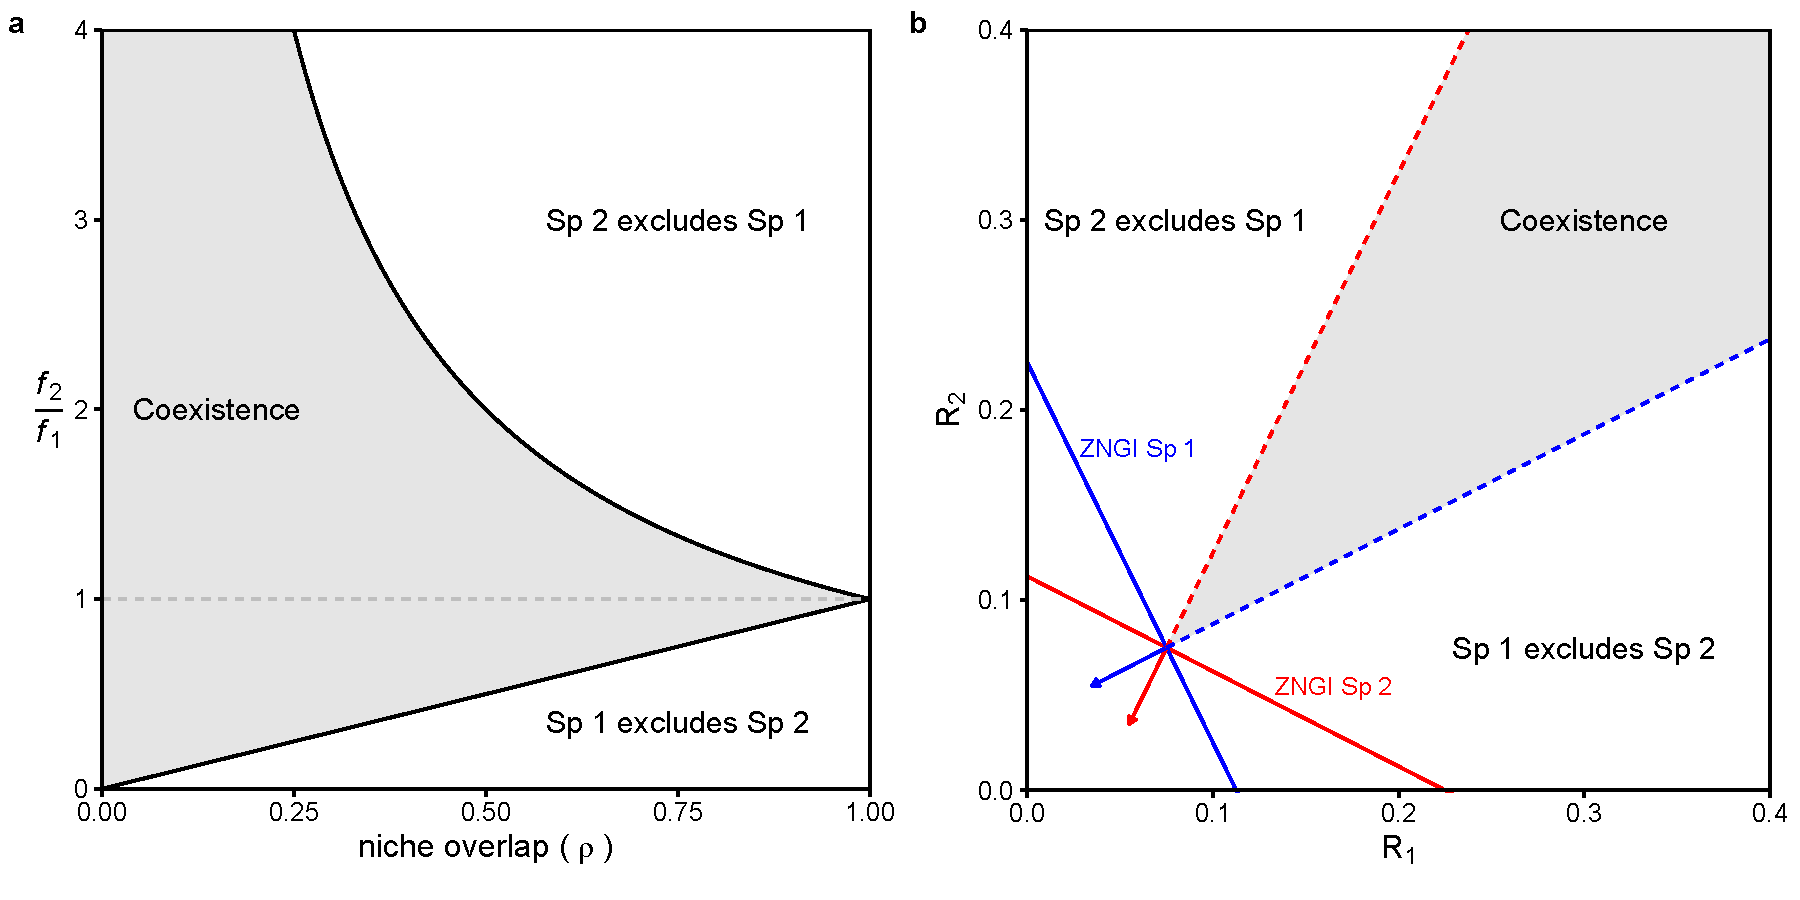
\includegraphics[width=15cm]{Chapter2/conceptfig.pdf}}
\caption[Graphical illustration of the criteria for coexistence under modern coexistence theory and contemporary niche theory.]
	{\hspace{1mm}Graphical illustration of the criteria for coexistence under modern coexistence theory (a) and contemporary niche theory (b). In (a) the lower and upper bounding black lines denote the point where the fitness ratio is equal to niche overlap and the inverse of niche overlap, respectively. Thus, according to the inequality $\rho < f_{2}/f_{1} < 1/\rho$, two species can coexist in the shaded region but exclude each other above or below these bounding lines. The asymmetry in (a) is due to the y-axis being a ratio, and therefore would appear symmetrical on a log scale i.e., contrary to their appearance on the ratio scale, the unshaded regions of parameter space corresponding to exclusion are equal in size for both species. In (b) coexistence of two species competing for two substitutable resources depends on three criteria: intersecting ZNGIs (solid red and blue lines connecting the x- and y-axes); each species having a greater impact on the resource from which it most benefits (impact vectors denoted by the red and blue arrows); and a resource supply ratio that is intermediate to the inverse of the impact vectors (dashed red and blue lines).}
\label{fig:conceptfig}
\end{figure}



\newpage
\begin{figure}[h!]
\centering
\makebox[\textwidth][c]{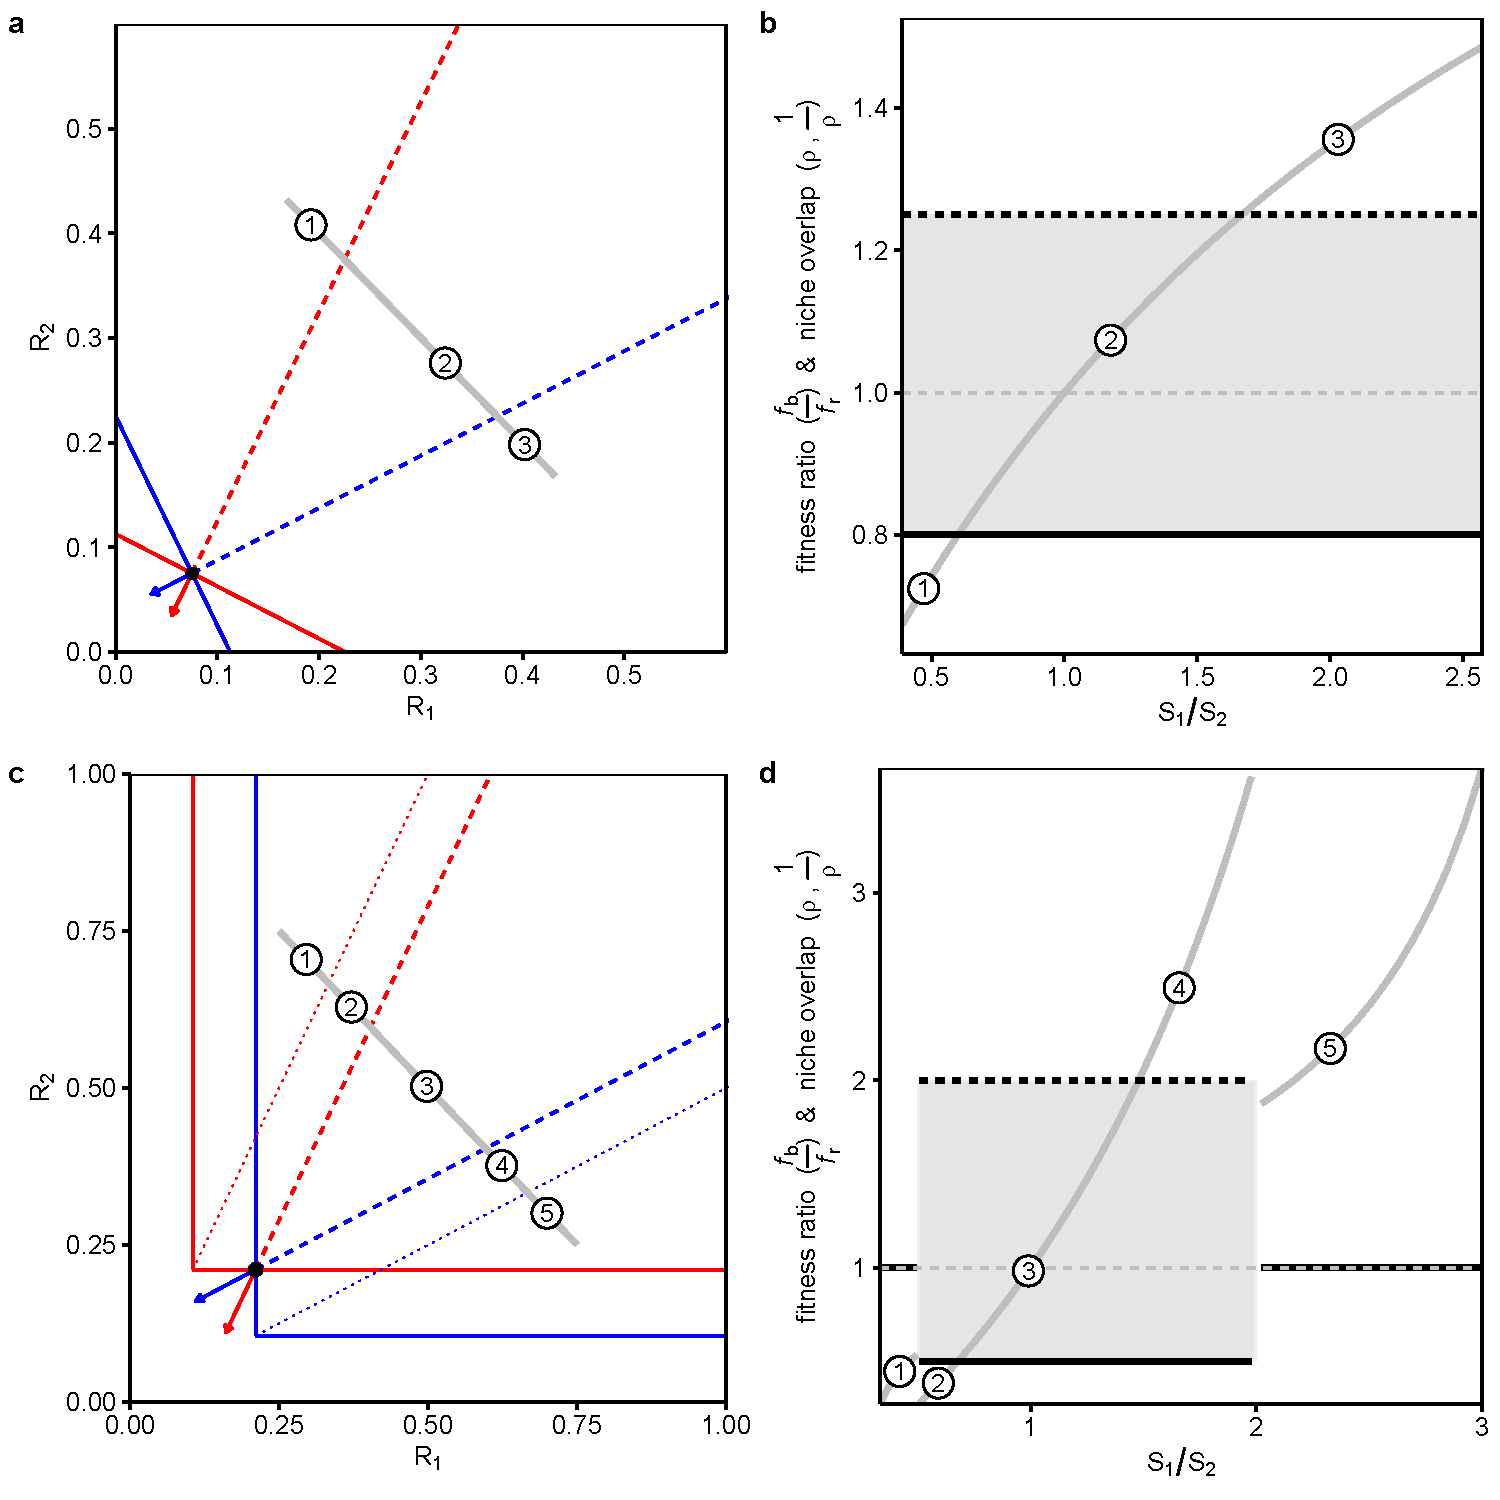
\includegraphics[width=12cm]{Chapter2/supply-ms-fig-flippedcols.pdf}}
\caption[Translating changing resource supply ratios in contemporary niche theory into the equalizing and stabilizing terms of modern coexistence theory, under pairwise competition for substitutable and essential resources.]
	{\hspace{1mm}Translating changing resource supply ratios in contemporary niche theory (a \& c) into the equalizing and stabilizing terms of modern coexistence theory (b \& d), under pairwise competition for substitutable (a \& b) and essential resources (c \& d). In (a) and (c), the solid red and blue lines are the ZNGIs for each species; the solid lines with arrow heads are the respective impact vectors; and the dashed lines are the inverse of the impact vectors, defining regions of stable coexistence. The additional dotted lines in (c) denote the regions in which species switch from being limited by different resources (above blue and below red) to being limited by the same resource (below blue or above red). In (b) and (d), the x-axis represents the resource ratio moving along the grey lines in (a) and (c) from top left to bottom right. The y-axis gives the values of the fitness ratio, $f_{b}/f_{r}$ (solid grey line), and the degree of niche overlap, $\rho$ (solid black line) and $1/\rho$ (dashed black line). The grey shaded area indicates the coexistence region, where $\rho<f_{b}/f_{r}<1/\rho$. For reference, equal fitness, where $f_{b}/f_{r}=1$, is illustrated by the horizontal dashed grey line. Numbers 1-3 in (a) and 1-5 in (c) correspond to the respective numbers in (b) and (d).}
\label{fig:supply-ms-fig}
\end{figure}



\newpage
\begin{figure}[h!]
\centering
\makebox[\textwidth][c]{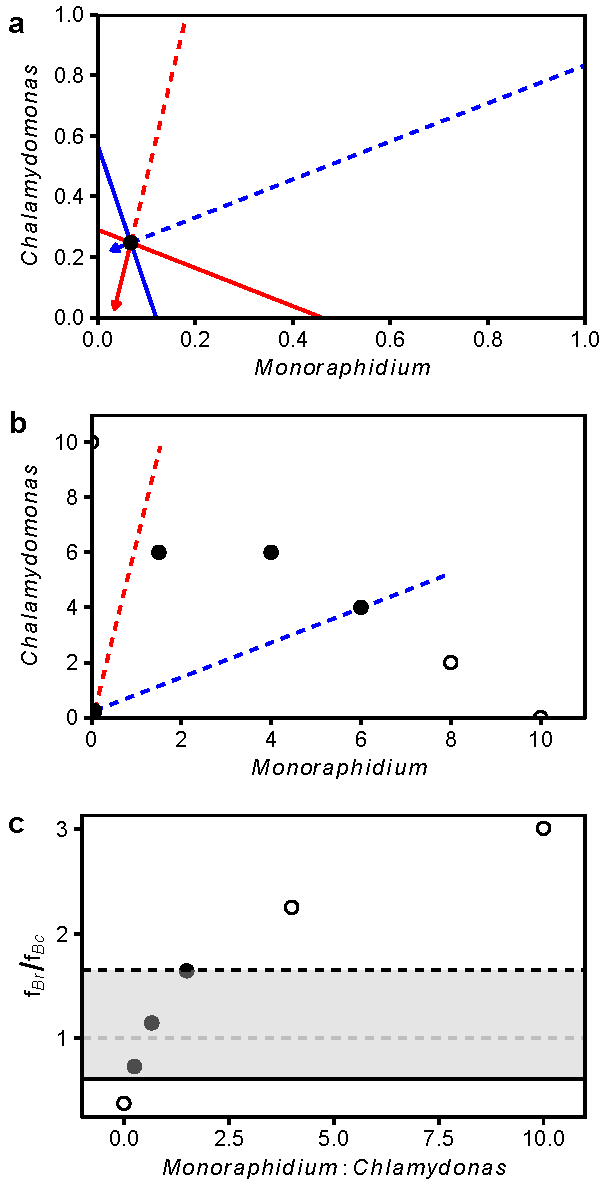
\includegraphics[width=7cm]{Chapter2/Box2-fig-Rothhaupt-colswitch.pdf}}
\caption[Illustrating the equivalence of predictions from contemporary niche theory and modern coexistence theory using data from \citet{Rothhaupt1988}.]
	{\hspace{1mm}Illustrating the equivalence of predictions from contemporary niche theory and modern coexistence theory using data from \citet{Rothhaupt1988}. In the top panel (a) ZNGIs and consumption vectors for \textit{B. rubens} and \textit{B. calyciflorus} are shown in blue and red respectively. The relationship between different supply point ratios (circles) and the inverse of the consumption vectors are shown in the middle panel (b), where filled circles indicate supply points where both species are predicted to coexist and empty circles indicate regions where one species is predicted to competitively exclude the other. The corresponding niche overlap, $\rho$, and fitness ratio, $f_{Br}/f_{Bc}$, values are shown in the bottom panel (c). Solid and dashed black lines indicate $\rho$ and $1/\rho$ respectively; dashed grey line indicates equal fitness; filled circles indicate regions of coexistence where  $\rho < f_{Br}/f_{Bc} < 1/\rho$; empty circles indicate regions of competitive exclusion.}
\label{fig:Box2-fig-Rothhaupt}
\end{figure}



\newpage
\begin{figure}[h!]
\centering
\makebox[\textwidth][c]{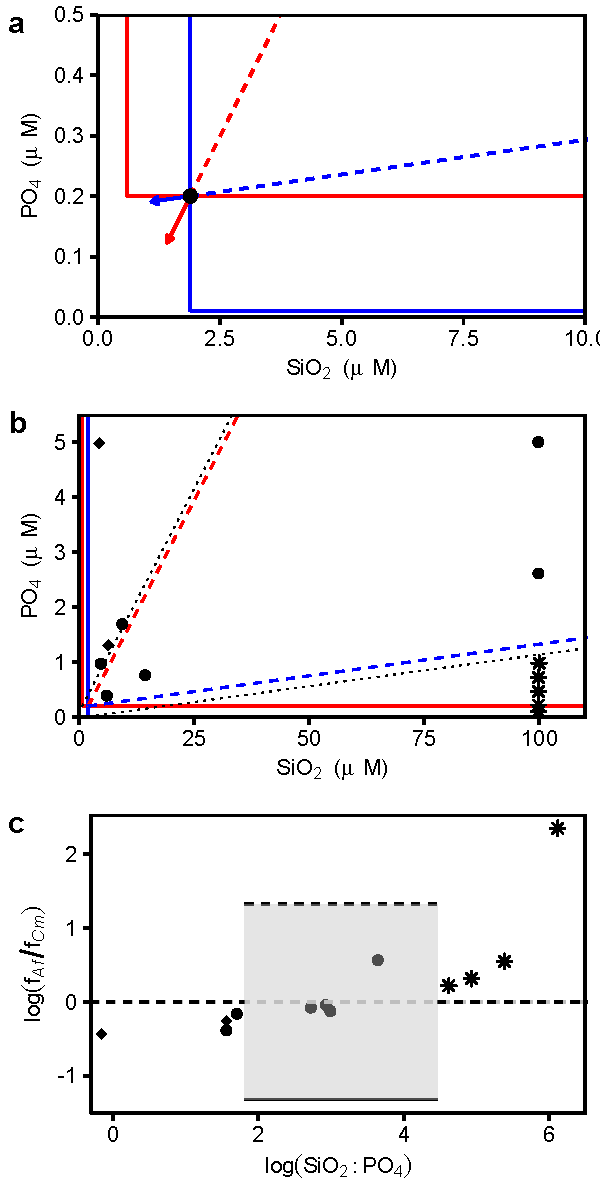
\includegraphics[width=7cm]{Chapter2/Box2-fig-Tilman-colswitch.pdf}}
\caption[Illustrating the equivalence of predictions from contemporary niche theory and modern coexistence theory using data from \citet{Tilman1977, tilman1982}.]
	{\hspace{1mm} Illustrating the equivalence of predictions from contemporary niche theory and modern coexistence theory using data from \citet{Tilman1977, tilman1982}. In the top panel (a) ZNGIs and consumption vectors for \textit{Asterionella} and \textit{Cyclotella}) are shown in blue and red respectively. The relationship between different supply point ratios and the inverse of the consumption vectors are shown in the middle panel (b). Corresponding with Fig. 31.A of \citet{tilman1982}, the supply point symbols indicate the outcome of competition experiments where stars denote the exclusion of \textit{Cyclotella} by \textit{Asterionella}, dots denote coexistence, and diamonds denote the exclusion of \textit{Asterionella} by \textit{Cyclotella}. The corresponding niche overlap, $\rho$, and fitness ratio, $f_{Af}/f_{Cm}$, values are shown in the bottom panel (c). Solid and dashed black lines indicate $\rho$ and $1/\rho$ respectively; dashed grey line indicates equal fitness; shaded area indicates region of coexistence where  $\rho < f_{Af}/f_{Cm} < 1/\rho$. To aid visualization, both axes in (c) have been log-transformed.}
\label{fig:Box2-fig-Tilman}
\end{figure}



\newpage
\begin{figure}[h!]
\centering
\makebox[\textwidth][c]{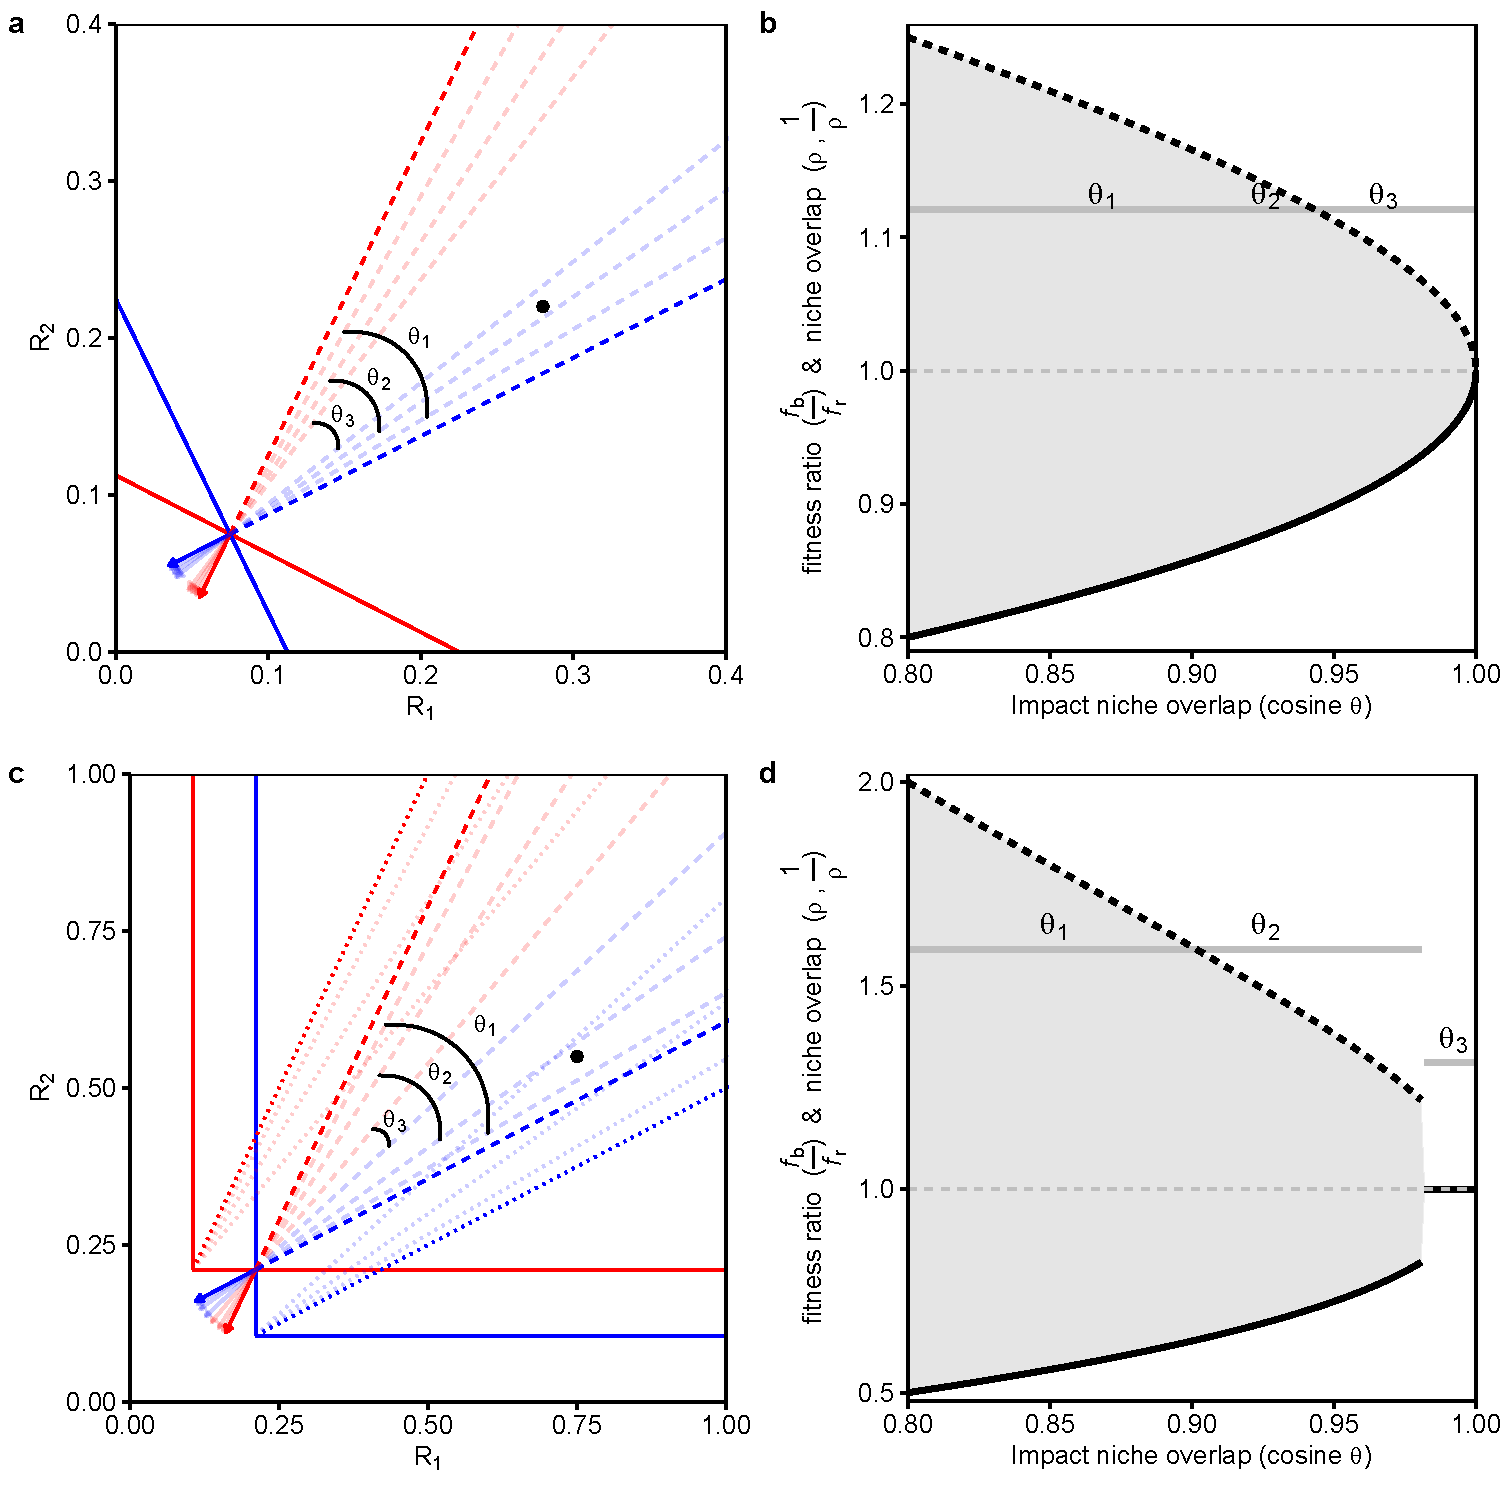
\includegraphics[width=12cm]{Chapter2/impact-ms-fig-flippedcols.pdf}}
\caption[Translating changing impact niche overlap in contemporary niche theory into the equalizing and stabilizing terms of modern coexistence theory, under pairwise competition for substitutable and essential resources.]
	{\hspace{1mm}Translating changing impact niche overlap in contemporary niche theory (a \& c) into the equalizing and stabilizing terms of modern coexistence theory (b \& d), under pairwise competition for substitutable (a \& b) and essential resources (c \& d). In (a) and (c), the solid red and blue lines are the ZNGIs for each species; the solid lines with arrow heads are the respective impact vectors; and the dashed lines are the inverse of the impact vectors, defining regions of stable coexistence. The additional dotted lines in (c) denote the regions in which species switch from being limited by different resources (above blue and below red) to being limited by the same resource (below blue or above red). In (b) and (d), the x-axis represents the impact niche overlap starting in the position given by the bold dashed lines and ending at complete overlap. The y-axis gives the values of the fitness ratio, $f_{b}/f_{r}$ (solid grey line), and the degree of niche overlap, $\rho$ (solid black line) and $1/\rho$ (dashed black line). The grey shaded area indicates the coexistence region, where $\rho<f_{b}/f_{r}<1/\rho$. For reference, equal fitness, where $f_{b}/f_{r}=1$, is illustrated by the horizontal dashed grey line. The angles given by $\theta_{1-3}$ in (a) and (c) correspond to the respective $\theta_{1-3}$ in (b) and (d). Impact niche overlap is defined here as the cosine of the angle between species' impact vectors, $\mathit{cosine}\ \theta = \frac{c_{11}c_{21}+c_{12}c_{22}}{\sqrt{c_{11}^{2}+c_{12}^{2}}\times \sqrt{c_{21}^{2}+c_{22}^{2}}}$, where $\left (c_{i1}, c_{i2}\right )$ is the consumption vector for species $\mathit{i}$ (see Appendix A.1 and Box 1 for parameter definition).}
\label{fig:impact-ms-fig}
\end{figure}



\newpage
\begin{figure}[h!]
\centering
\makebox[\textwidth][c]{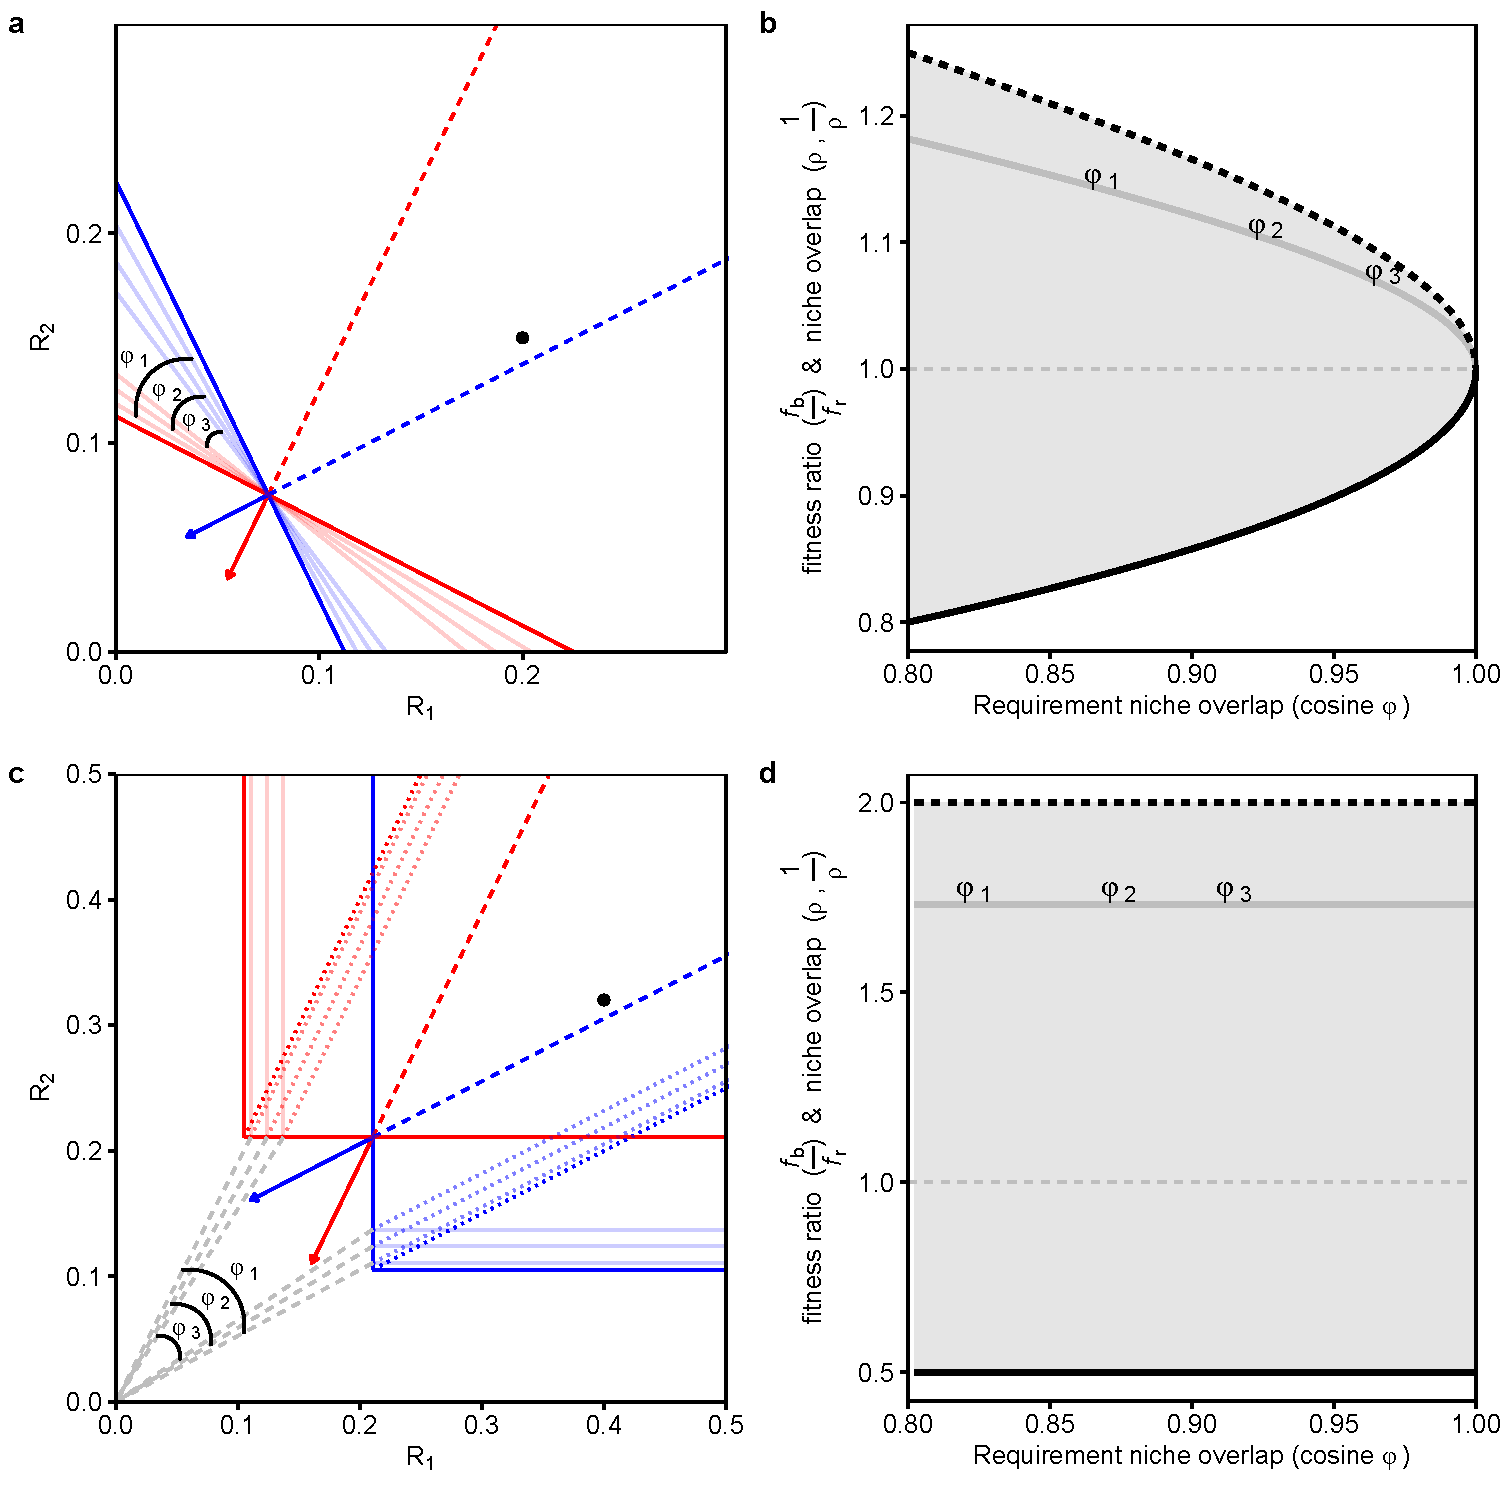
\includegraphics[width=12cm]{Chapter2/require-ms-fig-fixedequilibrium-flippedcols.pdf}}
\caption[Translating changing requirement niche overlap in contemporary niche theory into the equalizing and stabilizing terms of modern coexistence theory, under pairwise competition for substitutable and essential resources.]
	{\hspace{1mm}Translating changing requirement niche overlap in contemporary niche theory (a \& c) into the equalizing and stabilizing terms of modern coexistence theory (b \& d), under pairwise competition for substitutable (a \& b) and essential resources (c \& d). In (a) and (c), the solid red and blue lines are the ZNGIs for each species; the solid lines with arrow heads are the respective impact vectors; and the dashed lines are the inverse of the impact vectors, defining regions of stable coexistence. The additional dotted lines in (c) denote the regions in which species switch from being limited by different resources (above blue and below red) to being limited by the same resource (below blue or above red). In (b) and (d), the x-axis represents the requirement niche overlap starting in the position given by the solid bold ZNGIs and ending at complete overlap. The y-axis gives the values of the fitness ratio, $f_{b}/f_{r}$ (solid grey line), and the degree of niche overlap, $\rho$ (solid black line) and $1/\rho$ (dashed black line). The grey shaded area indicates the coexistence region, where $\rho<f_{b}/f_{r}<1/\rho$. For reference, equal fitness, where $f_{b}/f_{r}=1$, is illustrated by the horizontal dashed grey line. The angles given by $\varphi_{1-3}$ in (a) and (c) correspond to the respective $\varphi_{1-3}$ in (b) and (d). Requirement niche overlap for substitutable resources is defined here as the cosine of the angle between species' ZNGIs, $\mathit{cosine}\ \phi  = \frac{w_{12}w_{22}+w_{11}w_{21}}{\sqrt{w_{11}^{2}+w_{12}^{2}}\times \sqrt{w_{21}^{2}+w_{22}^{2}}}$, where $\frac{-w_{i1}}{w_{i2}}$ is the ZNGI's slope for species $\mathit{i}$. Requirement niche overlap for essential resources is defined as the cosine of the angle between two lines from the origin to the corner of each ZNGI, $\mathit{cosine}\ \phi  = \frac{R_{11}^{*}R_{21}^{*}+R_{12}^{*}R_{22}^{*}}{\sqrt{R_{11}^{*2}+R_{12}^{*2}}\times \sqrt{R_{21}^{*2}+R_{22}^{*2}}}$, where $\left (R_{i1}^{*}, R_{i2}^{*}\right )$ is the coordinate of corner of the ZNGI for species $\mathit{i}$ (see main text, Appendix A.1 and Box 1 for parameter definition).}
\label{fig:require-ms-fig-fixedequilibrium}
\end{figure}



\clearpage 
\begin{tcolorbox}[breakable, leftright skip=-0.5cm]
\subsection*{Box 1: Deriving niche overlap and fitness differences in terms of consumer-resource parameters}
In order to explore the analytical relationship between modern coexistence theory \citep{Chesson2000} and contemporary niche theory \citep{Chase2003} we first translated a consumer-resource model into Lotka--Volterra form following \citet[][Ch.~7]{tilman1982}. This was done by solving the equilibrium of the consumer-resource model, and rearranging the equilibrium algebraically \citep[for an alternative approach see][]{Meszenaz2006, Barabas2014}. A summary of the mathematical derivation for substitutable resources is provided here, and in full for both substitutable and essential resources in Appendix A.1.
\par


Tilman's (\citeyear{tilman1982}) consumer-resource model consists of two resources ($R_{1}$ and $R_{2}$) that are perfectly nutritionally substitutable for two consumers ($N_{1}$ and $N_{2}$). By setting the right hand side of the consumer equations to zero, \citet{tilman1982} solved for the equilibrium and rearranged the consumer equilibrium density to a form comparable to the Lotka--Volterra model (i.e., $N_{1}^{*}=\frac{1}{a_{11}}-\frac{a_{12}}{a_{11}}N_{2}^{*}$ and $N_{2}^{*}=\frac{1}{a_{22}}-\frac{a_{21}}{a_{22}}N_{1}^{*}$). The equilibrium density for $N_{1}$ and $N_{2}$ can be subsequently written as:

\begin{equation}
N_1^* = \left[ {\frac{{D\left( {{S_2} + \frac{{{w_{11}}}}{{{w_{12}}}}{S_1} - {B_1}} \right)}}{{{c_{12}} + {c_{11}}\frac{{{w_{11}}}}{{{w_{12}}}}}}} \right] - \left[ {\frac{{{c_{22}} + {c_{21}}\frac{{{w_{11}}}}{{{w_{12}}}}}}{{{c_{12}} + {c_{11}}\frac{{{w_{11}}}}{{{w_{12}}}}}}} \right]N_2^*
\tag{2.4.1}\label{eq:2.4.1}
\end{equation}
\begin{equation}
N_2^* = \left[ {\frac{{D\left( {{S_2} + \frac{{{w_{21}}}}{{{w_{22}}}}{S_1} - {B_2}} \right)}}{{{c_{22}} + {c_{21}}\frac{{{w_{21}}}}{{{w_{22}}}}}}} \right] - \left[ {\frac{{{c_{12}} + {c_{11}}\frac{{{w_{21}}}}{{{w_{22}}}}}}{{{c_{22}} + {c_{21}}\frac{{{w_{21}}}}{{{w_{22}}}}}}} \right]N_1^*.
\tag{2.4.2}\label{eq:2.4.2}
\end{equation}

\noindent Here, $r_{i}$ represents the maximum population growth rate for species $i$ ($i = $ 1 or 2) and $D$ represents the constant mortality of the consumers and turnover rate of resources. Per capita resource consumption rate of consumer $N_{i}$ on resource $R_{j}$ ($j = $ 1 or 2) is represented by $c_{ij}$, whereas $w_{ij}$ represents a weighting factor that converts availability of $R_{j}$ into its value for consumer $N_{i}$. Following a Monod growth model, $k_{i}$ is the half-saturation constant for $N_{i}$ resource consumption, and $T_{i}$ is the minimum amount of total resource required for $N_{i}$ to grow. Finally, $S_{1}$ and $S_{2}$ represents the resource supply concentration for $R_{1}$ and $R_{2}$, respectively.
\par


Eqns.~\ref{eq:2.4.1} and \ref{eq:2.4.2} consists of two parts. The first bracket represents a density-independent component with only $N_{1}$- and $N_{2}$-related parameters and are the algebraic equivalent of $\frac{1}{a_{11}}$ and $\frac{1}{a_{22}}$, respectively. The second bracket represents a heterospecific density-dependent component that decreases with its competitors' density, and is the algebraic equivalent of $\frac{a_{12}}{a_{11}}$ and $\frac{a_{21}}{a_{22}}$ in the Lotka--Volterra model, respectively.
\par


Chesson defines niche overlap as $\rho=\sqrt {\frac{{{a_{12}}{a_{21}}}}{{{a_{11}}{a_{22}}}}}$ and average fitness difference of $N_{2}$ over $N_{1}$ as $\frac{{{f_2}}}{{{f_1}}} = \sqrt {\frac{{{a_{11}}{a_{12}}}}{{{a_{22}}{a_{21}}}}}$ \citep{Chesson2008b, Chesson2013ecosys}. Thus niche overlap for two consumers competing for substitutable resources can be expressed as:

\begin{equation}
\rho  = \sqrt {\frac{{{a_{12}}{a_{21}}}}{{{a_{11}}{a_{22}}}}}  = \sqrt {\frac{\left (
		c_{22} + c_{21}\frac{w_{11}}{w_{12}}\right )\left ( 
		c_{12} + c_{11}\frac{w_{21}}{w_{22}} \right )}{\left (
		c_{12} + c_{11}\frac{w_{11}}{w_{12}}\right )\left ( 
		c_{22} + c_{21}\frac{w_{21}}{w_{22}} \right )}} 
\tag{2.5.1}\label{eq:2.5.1}
\end{equation}
and the absolute fitness difference of $N_{2}$ over $N_{1}$ is:
\begin{equation}
\frac{{{f_2}}}{{{f_1}}} = \sqrt {\frac{{{a_{11}}{a_{12}}}}{{{a_{22}}{a_{21}}}}}  = \frac{\left (S_{2}+\frac{w_{21}}{w_{22}}S_{1}-B_{2}\right )}{\left (S_{2}+\frac{w_{11}}{w_{12}}S_{1}-B_{1}\right )}\sqrt {\frac{\left (
		c_{12} + c_{11}\frac{w_{11}}{w_{12}}\right )\left ( 
		c_{22} + c_{21}\frac{w_{11}}{w_{12}} \right )}{\left (
		c_{22} + c_{21}\frac{w_{21}}{w_{22}}\right )\left ( 
		c_{12} + c_{11}\frac{w_{21}}{w_{22}} \right )}}.
\tag{2.5.2}\label{eq:2.5.2}
\end{equation}
\end{tcolorbox}



\clearpage
\begin{tcolorbox}[breakable, leftright skip=-0.5cm]
\subsubsection*{Box 2: Empirical tests of consumer-resource competition through the lens of modern coexistence theory}
In order to illustrate further the transformation between contemporary niche theory and modern coexistence theory, we extracted data from two seminal experimental works on resource competition, \citet{Rothhaupt1988} and \citet{Tilman1977}. 
\par


\citet{Rothhaupt1988} investigated the effect of modifying the ratio of two substitutable resources on the competitive dynamics of two species of herbivorous zooplankton, the rotifers \textit{Brachionus rubens} and \textit{B. calyciflorus}. To quantity the parameters defining each species' ZNGI and consumption vectors, \citet{Rothhaupt1988} first measured the per capita growth rate of \textit{B. rubens} and \textit{B. calyciflorus} across a range of concentrations of two algae species (\textit{Monoraphidium minutum} and \textit{Chlamydonas sphaeroides}). These were subsequently used to make predictions on the outcomes of competition between the two rotifers at different supply ratios of the two resources and at two dilution rates (the nutrient independent mortality rate in a chemostat).
\par


We extracted the relevant parameters at the lower dilution rate (either from the text or from figure 2a) and used these to quantify Chesson's niche overlap and fitness ratio terms following the approach outlined in Box 1. Fig.~\ref{fig:Box2-fig-Rothhaupt}a shows each species' ZNGI and associated consumption vector, and corresponds with Figure 2a of \citet{Rothhaupt1988}. Notably the intersecting ZNGIs and positively correlated consumption vectors satisfy two of the three criteria for stable coexistence. Fig. \ref{fig:Box2-fig-Rothhaupt}b, which is drawn on a different scale to Fig. \ref{fig:Box2-fig-Rothhaupt}a, shows the manipulated resource supply ratios, where black dots satisfy the third criteria for stable coexistence, intermediate supply rates. Fig. \ref{fig:Box2-fig-Rothhaupt}c shows the equivalent coexistence predictions when translated into Chesson's niche overlap and fitness ratio. In accordance with the logic of the main text, manipulating resource supply ratio only affects fitness differences, and the regions of stable coexistence correspond with those identified by Tilman's graphical method. In subsequent competition experiments, \citet{Rothhaupt1988} found the results to be in agreement with theoretical predictions in all but one of the scenarios outlined above.
\par


Tilman (\citeyear{Tilman1977, tilman1982}) investigated the effect of modifying the ratios of two essential resources, phosphate and silicate, on the coexistence of two algal species, \textit{Asterionella formosa} and \textit{Cyclotella meneghiniana}. As for the Rothhaupt data, we used the parameters given in \cite{Tilman1977} and extracted the supply point ratios from Fig. 31.A of \citet{tilman1982} to quantify Chesson's niche overlap and fitness ratio terms. Fig. \ref{fig:Box2-fig-Tilman}a shows a zoomed-in view of each species' ZNGIs and impact vectors. Fig. \ref{fig:Box2-fig-Tilman}b, which corresponds with Fig. 31.A of \citet{tilman1982}, shows the position of the resource supply points and predicted outcomes of competition. When translated into Chesson's niche overlap and fitness ratio terms (Fig. \ref{fig:Box2-fig-Tilman}c) we see that the four supply points compatible with coexistence in Fig. \ref{fig:Box2-fig-Tilman}b all correspond with fitness ratios that are bounded by $\rho$ \& $1/\rho$. As highlighted in the main text, all of the supply points that fall outside the coexistence region are sufficiently extreme such that both species are limited by the same resource. This is reflected in the superimposition of $1/\rho$ and $\rho$ in Fig. \ref{fig:Box2-fig-Tilman}c. The results of subsequent competition experiments were in agreement with all but two of the predictions, where both species coexisted despite falling just outside the coexistence region identified in Fig. \ref{fig:Box2-fig-Tilman}b.
\par


Note that the equivalence of the coexistence predictions in both examples is a natural result of their deriving from the same underlying data. It would be valuable to conduct a more thorough comparative study using data collected independently for analysis under each framework, where inconsistent predictions could serve to highlight inappropriate assumptions.
\end{tcolorbox}
